
\documentclass[a4paper,12pt]{article}
\usepackage[a4paper,top=1.3cm,bottom=2cm,left=1.5cm,right=1.5cm,marginparwidth=0.75cm]{geometry}
\usepackage{cmap}					
\usepackage[warn]{mathtext} 		
\usepackage[T2A]{fontenc}			
\usepackage[utf8]{inputenc}			 
\usepackage[english,russian]{babel}	
\usepackage{longtable}
\usepackage{float}
\restylefloat{table}
\usepackage{graphicx}
\usepackage{tabularx}
\usepackage{hyperref}
\usepackage[rgb]{xcolor}
\usepackage{amsmath,amsfonts,amssymb,amsthm,mathtools} 
\mathtoolsset{showonlyrefs=true}
\usepackage{euscript}
\usepackage{mathrsfs}
\date{\today}
\begin{document}

\begin{titlepage}
	\begin{center}
		{\large МФТИ}
	\end{center}
	\begin{center}
		{\large ФРКТ}
	\end{center}
	
	
	\vspace{4.5cm}
	{\huge
		\begin{center}
			{\bf Лабораторная работа 5.10.1}\\
			Электронный парамагнитный резонанс.
		  
		

		\end{center}
	}
	\vspace{9cm}
	\begin{flushright}
		{\LARGE  $\newline$Добровольская Ксеня$\newline$Гаврилин Илья$\newline$
			\vspace{0.2cm}
			Б01-110$\newline$}
	\end{flushright}
	\vspace{8cm}
	
\end{titlepage}

\section{Аннотация}


  В данной работе был исследован электронный парамагнитный резонанс в молекуле ДФПГ. Измерены:
  
  \textbf{Ширина линии резонансного поглощения}, ее значение составило $\Delta B = 0.22$ мТл. 
  
  \textbf{g-фактор электрона}, значение которого составило g = 1.98. Данное значение совпадает с точностью 1\% с табличным значением для свободного электрона $g_{\text{своб}}= 2.0036$.                                                      

  
\section{Теоретические сведения}

	Энергетический уровень электрона в присутствии магнитного поля с индукцией $B$ расщепляется на два подуровня, расстояние между которыми равно 


\[	\Delta E = E_2 - E_1 = 2\mu B_0.\]
		
	Здесь $\mu$ -- абсолютная величина проекции магнитного момента на направление поля.
	
	Между этими двумя уровнями возможны переходы. Эти переходы могут возбуждаться внешним высокочастотным электромагнитным полем, если оно имеет нужную частоту и нужное направление.
	
	Резонансное значение частоты определяется из очевидной формулы:

  \[	\hbar \omega_0 = \Delta E.\]

	При переходе с нижнего на верхний уровень энергии электрон поглощает квант электромагнитной энергии, а при обратном переходе такой же квант излучается. Возбуждение электронных резонансных переходов электромагнитным полем, имеющим частоту $\omega_0$, носит название электронного парамагнитного резонанса (ЭПР).
	
	В настоящей работе необходимо получить сигнал ЭПР на кристаллическом дифенилпикрилгидразиле (ДФПГ) и определить значение $g$-фактора для электрона. Как известно, связь между магнитным моментом $\mu$ электрона и его механическим моментом $\mathbf{M}$ выражается через гиромагнитное отношение $\gamma$ с помощью формулы

   \[ \mu = \gamma M.\]

	Если магнитный момент частицы измерять в магнитонах Бора, а механический - в $\hbar$, то их связь можно записать через $g$-фактор:

	 \[ \frac{\mu}{\mu_\text{Б}} = g \frac{M}{\hbar} = g \frac{s\hbar}{\hbar} = gs = \frac{\hbar \omega_0}{2 B_0 \mu_\text{Б}}\]

,где $s = 1/2$ -- спин электрона

 
 
	Значит g-фактор:

	\[	g = \frac{\hbar \omega_0}{\mu_\text{Б} B_0}.\]
	

\section{Экспериментальная установка} 
   
   
Схема экспериментальной установки приведена на рис.1.

    \begin{figure}[H]
  \begin{center}
    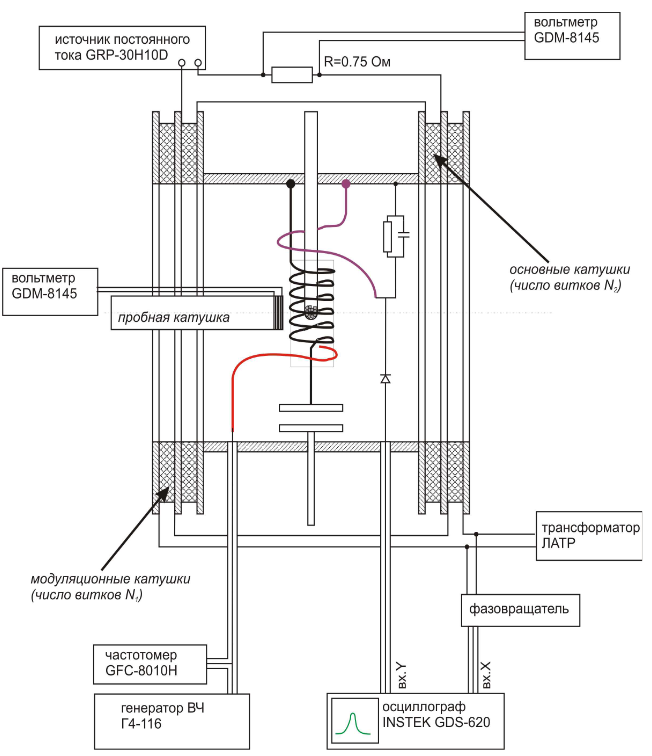
\includegraphics[width=10cm]{ex1.png}
    \caption{Схема экспериментальной установки.}
    \label{fig:}
  \end{center}
\end{figure}
 
	
Схема установки представлена на Рис. 1. Образец (порошок ДФПГ) в стеклянной ампуле помещается внутрь катушки индуктивности, входящей в состав колебательного контура. Входящий в состав контура конденсатор состоит из двух пластин, разделённых воздушным зазором, одна из пластин может перемещаться поворотом штока. Колебания в контуре возбуждаются антенной, соединённой с генератором высокой частоты (ВЧ) Г4-116. Амплитуда колебаний поля в катушке индуктивности
измеряется по наводимой в петле связи ЭДС индукции. Высокочастотные колебания ЭДС
индукции в приёмном контуре детектируются диодом, измеряемая при помощи
осциллографа низкочастотная огибающая этого сигнала пропорциональна квадрату
амплитуды колебаний поля в катушке.\\
Постоянное магнитное поле создаётся пропусканием тока от источника постоянного тока через основные катушки. 


\section{Измерения и обработка результатов}

\textbf{Характеристики пробной катушки}

  \begin{table}[H]
\begin{center}
\begin{tabular}{|c|c|}
\hline N, \text{шт} &D, mm\\
\hline 44& 15.1\\
\hline
\end{tabular}
\end{center}
\end{table}
 
 \begin{enumerate}
    \item \textbf{Настройка ВЧ генератора на частоту колебательного контура.} Подстройкой частоты добиваемся максимальной амплитуды сигнала на экране осциллографа. Эта частота равна $f_0 =$162.700 МГц. Осциллограмма при настройке генератора изображена на рис.2.
        		    \begin{figure}[H]
  \begin{center}
    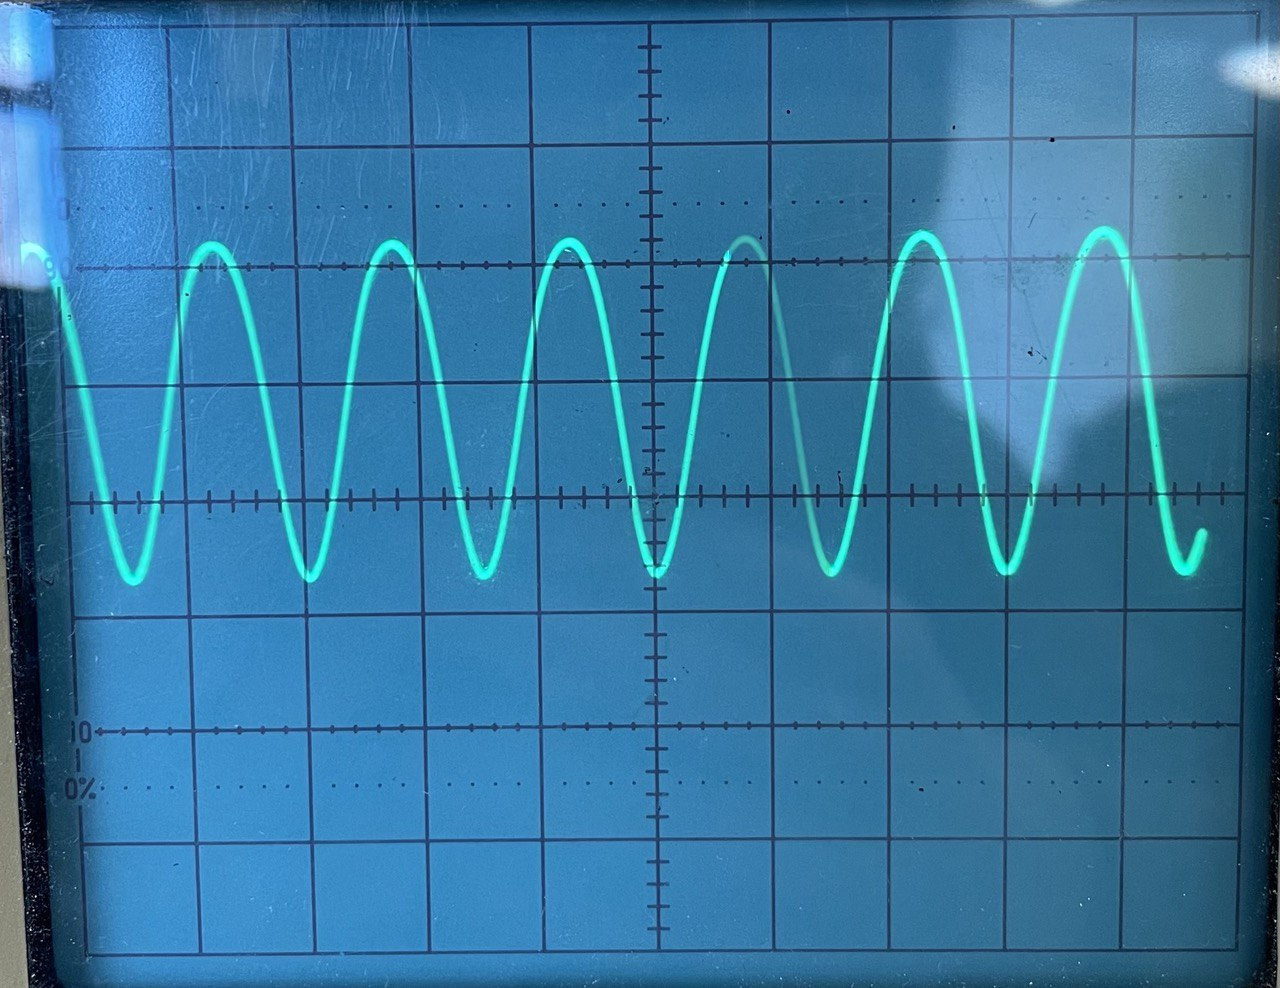
\includegraphics[width=12cm]{ex2.jpg}
    \caption{Осциллограмма при настройке генератора.}
    \label{fig:}
  \end{center}
\end{figure}

    \item \textbf{Наблюдение сигнала резонансного поглощения.} Для этого подключаем основные катушки к источнику постоянного тока, а модуляционные катушки к трансформатору ЛАТР. Подбираем величину постоянного магнитного поля в основных катушках так, чтобы наблюдался сигнал резонансного поглощения. Добиваемся эквидистантности пиков. 
  \newline 
  
  Зафиксированный сигнал изображен на рис. 3.
    
       		    \begin{figure}[H]
  \begin{center}
    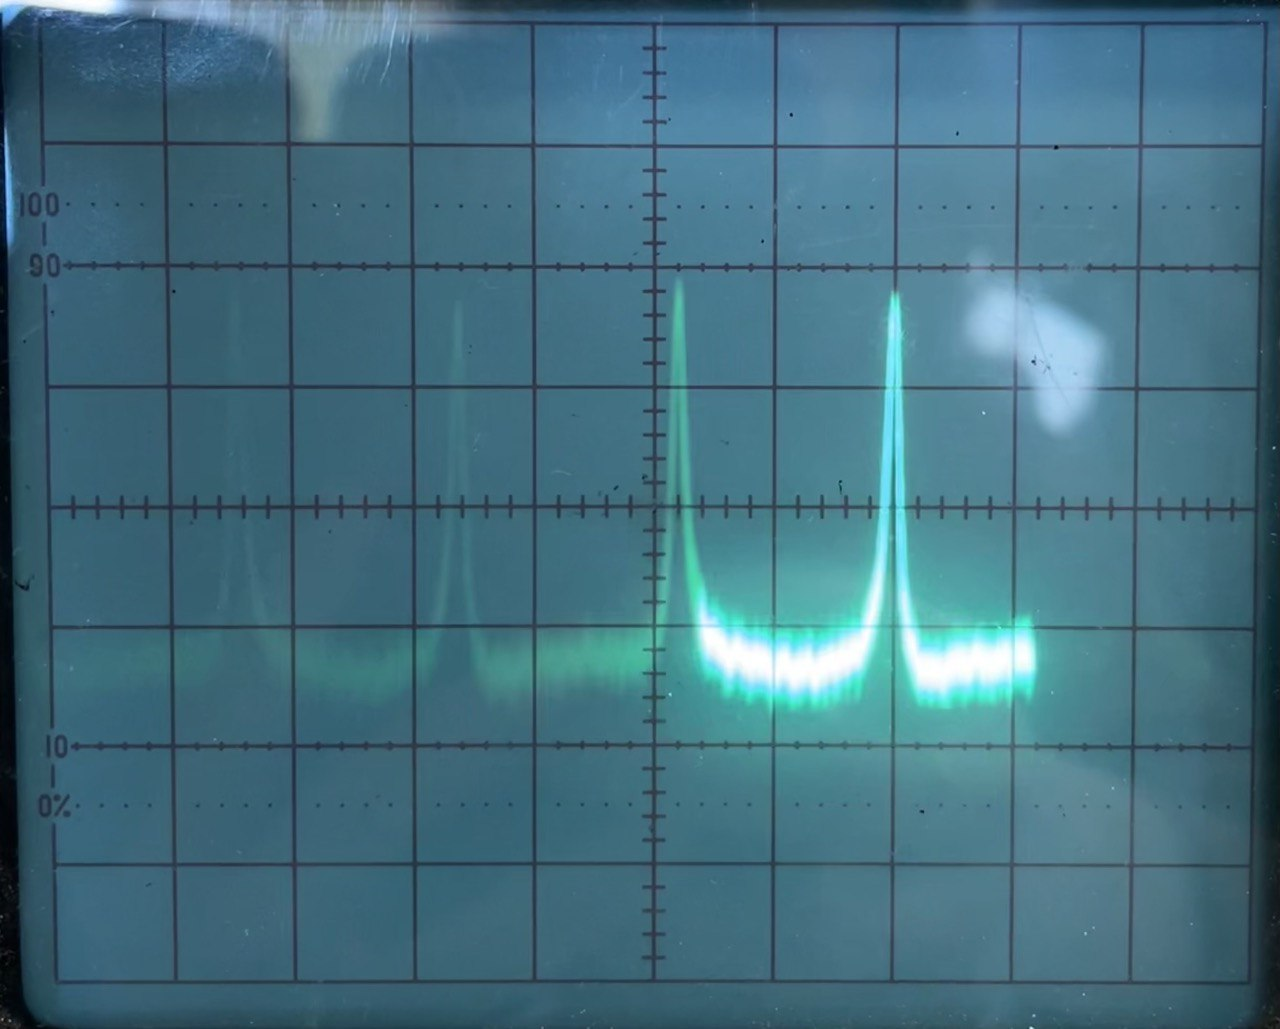
\includegraphics[width=12cm]{ex3.jpg}
    \caption{Осциллограмма сигнала поглощения при резонансном постоянном поле.}
    \label{fig:}
  \end{center}
\end{figure}
    
    Вносим пробную катушку в соленоид и измеряем ЭДС-индукции:
    
    $U = (14.55 \pm 0.01)$ мВ
    
    По этой величине можем рассчитать величину постоянного магнитного поля:
    
    \[U = N_{\text{проб}} S \omega B_0 =>  B_0 = \frac{U}{N_{\text{проб}} S \omega} = (5.88 \pm 0.01) \text{мТл}\]
    
    , где $S = \frac{\pi (D_{проб})^2}{4}$-- площадь сечения пробной катушки, $\omega = 2\pi \vartheta $ -- угловая частота переменного тока, $\vartheta $= 50 Гц.
    
 
% Это комментарий
%    		    \begin{figure}[H]
%  \begin{center}
%    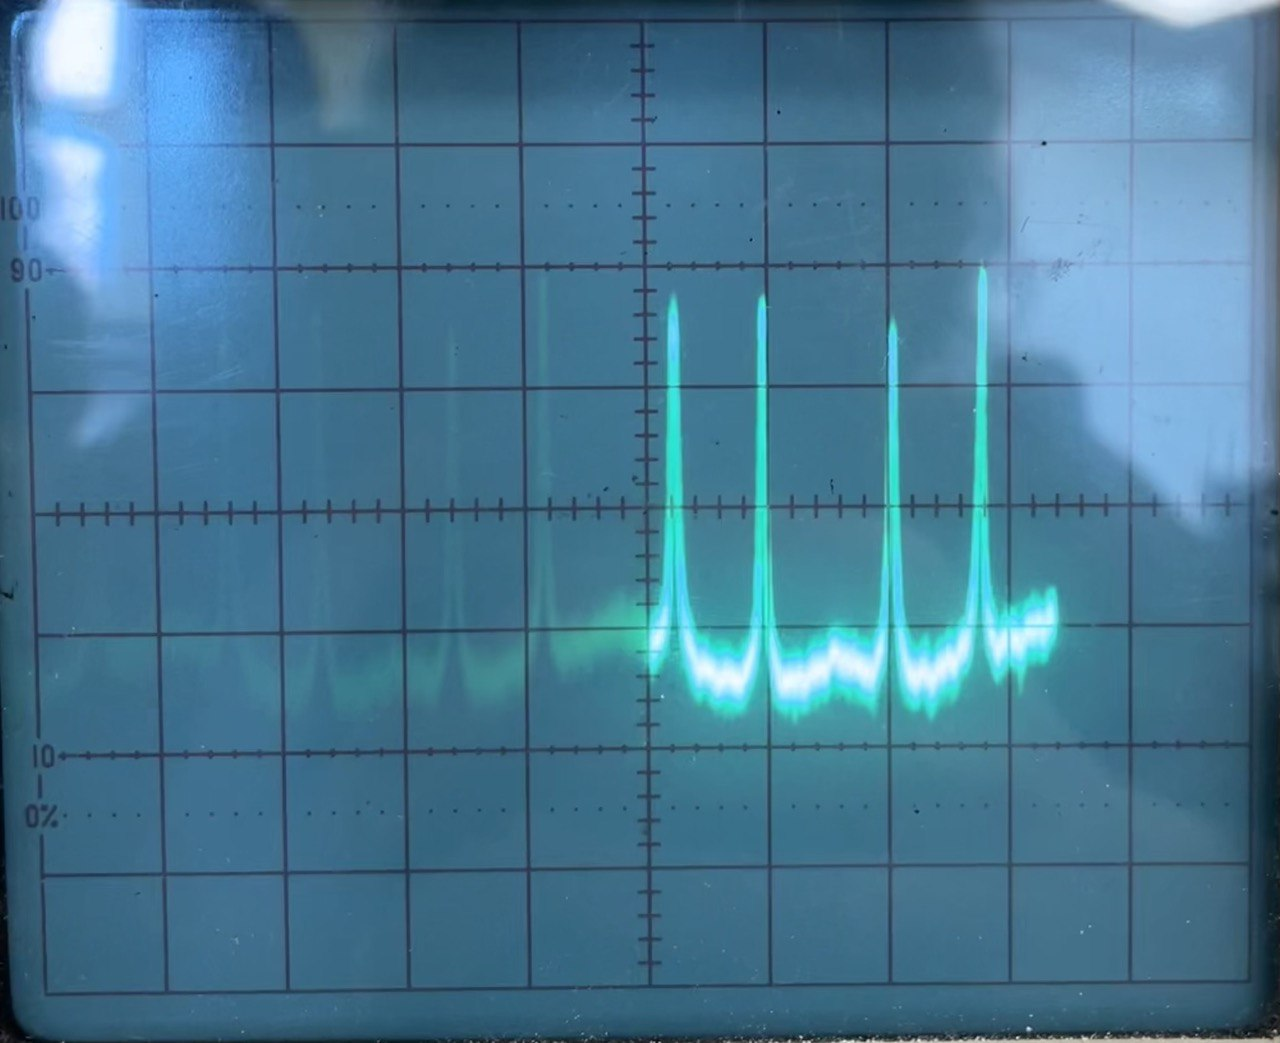
\includegraphics[width=12cm]{ex4.jpg}
%    \caption{А здесь в два раза чаще.}
%    \label{fig:}
%  \end{center}
%\end{figure}

   \item \textbf{Определение ширины линии поглощения.} Переводим осциллограф в режим XY-развертки.
   
    
   \textbf{X} - напряжение на модулирующих катушках
   
   \textbf{Y} - сигнал с детектора
   
   Добиваемся появления хорошо прорисованной линии резонансного поглощения. Подстройкой фазовращателя совмещаем два пика, соответствующих прохождению резонансного поглощения на растущем и падающем полупериодах модулирующего напряжения. Наблюдаемый сигнал изображен на рис.5. 
   
         \begin{figure}[H]
  \begin{center}
    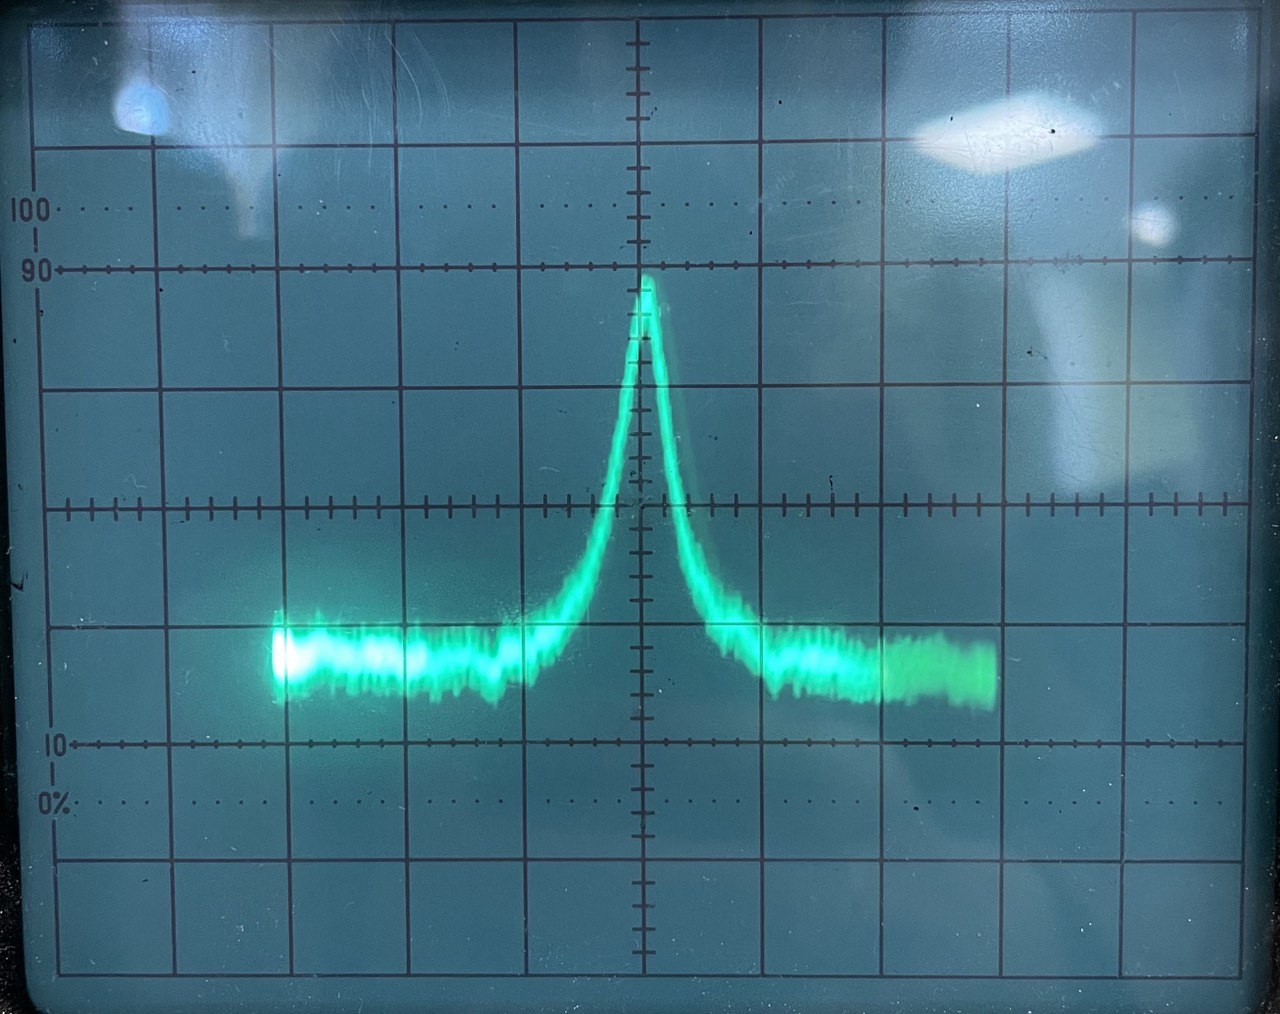
\includegraphics[width=12cm]{ex5.jpg}
    \caption{Линия резонансного поглощения в режиме XY-развертки.}
    \label{fig:}
  \end{center}
\end{figure}

   
    \item Для определения ширины линии ЭПР определим по экрану осцилографа полный размах поля $A_{0}$ и полную ширину кривой резонансного поглощения на полувысоте $A_{\frac{1}{2}}$. 
    
    $A_{0} = 6.0 \pm 0.2 $дел
    
    $A_{\frac{1}{2}} = 0.6 \pm 0.2$ дел
    
    При помощи пробной катушки определим амплитуду модуляции магнитного поля. Для этого внесем её внутрь соленоида. Переменное поле модуляционных катушек наводит в пробной катушке ЭДС индукции $\varepsilon $, по которой можно определить величину поля. Измеренное ЭДС индукции: 
    
    $\varepsilon = (3.88 \pm  0.01)$мВ
    
     \textbf{Амплитуда модулирующего поля}:
    
    $B_{\text{мод}} = \dfrac{2\sqrt{2} \varepsilon }{\pi^2 d^2_{\text{проб}} N_{\text{проб}}\vartheta } = (2.22 \pm 0.01)$ мТл
    
    , где $\vartheta $= 50 Гц -- частота модулирующего напряжения 


  Тогда  \textbf{ширина линии ЭПР}:
  
  $\Delta B = \frac{A_{\frac{1}{2}}}{A_{0}} B_{\text{мод}} = (0.22 \pm 0.07)$ мТл
    
    
		\item \textbf{Определение $g$-фактора}. По полученным данным определяем значение эффективного $g$-фактора исследуемого вещества ($\hbar = 1.054 * 10^{-34} \text{Дж с}, \mu_\text{Б} = 927.4 * 10^{-26} \text{Дж/Тл}$):
		
		\[g = \frac{\hbar \omega_0}{\mu_\text{Б} B_0} = \frac{\hbar 2 \pi f_0}{\mu_\text{Б} B_0} = (1.98 \pm 0.01)\]

	
\textbf{Табличное значение} g-фактора свободного электрона - $g_{\text{своб}} = 2.0036$. Отклонение от табличного значения - 1\%.
	\end{enumerate}



\section{Выводы}

В данной работе мы исследовали ЭПР в молекуле ДФПГ. Измерили 

\textbf{Ширину линии резонансного поглощения}, ее значение составило $\Delta B = 0.22$ мТл. 

\textbf{g-фактор электрона}, значение которого составило g = 1.98. Данное значение совпадает с точностью 1\% с табличным значением для свободного электрона $g_{\text{своб}} = 2.0036$, это свидетельствует о том, что ЭПР происходит на неспаренных электронах почти так же, как и на свободных.

\end{document}
	
